\chapter{Manual de usuario}

\section{Acceso a la aplicación}
La primera página que se carga de nuestra aplicación web es la que se refiere al login. En la imagen \ref{fig:login} podemos consultar el aspecto de dicha página. Observamos dos entradas de texto, una para insertar el nombre de usuario y otra para la contraseña. \\

Para usuarios que no estén registrados se presenta la opción de \textbf{Crear una nueva cuenta}, en la cual debemos rellenar los datos requeridos: nombre de usuario, dirección de correo electrónico, contraseña y confirmar contraseña. En la imagem \ref{fig:registro}

\begin{figure}[H]
	\centering
	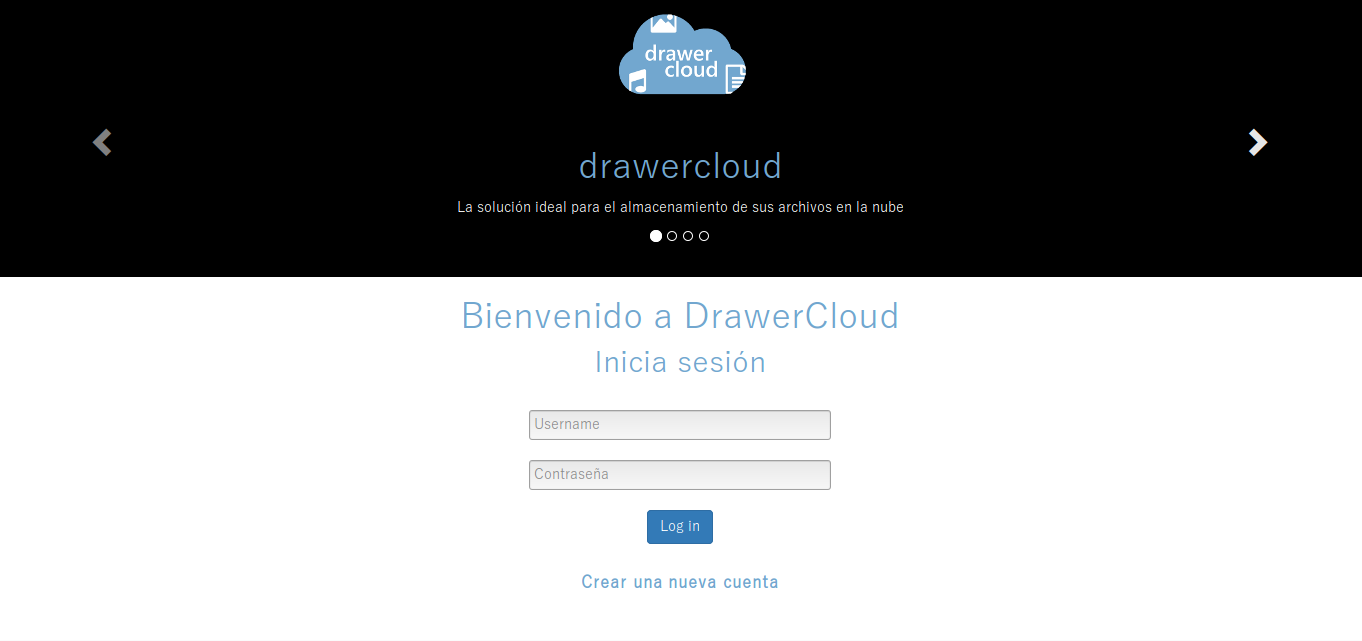
\includegraphics[width=1\textwidth]{imagenes/login}
	\caption{Acceso a la aplicación. Página de login}
	\label{fig:login}
\end{figure}

\begin{figure}[H]
	\centering
	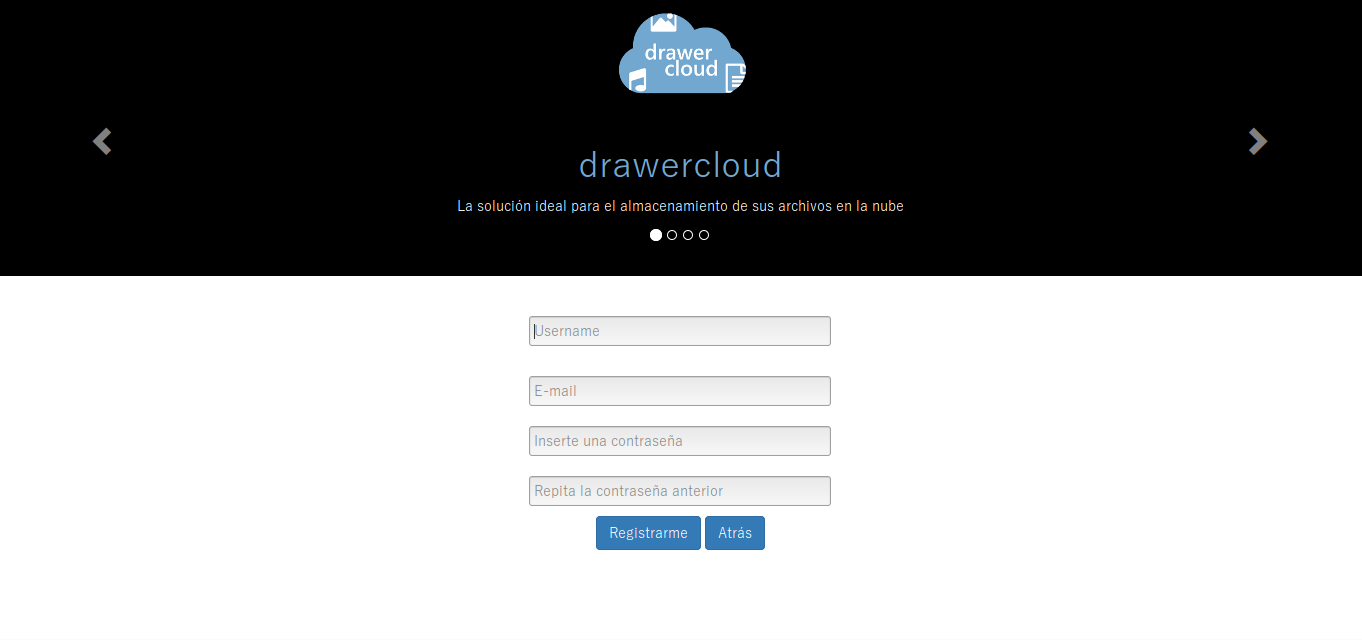
\includegraphics[width=1\textwidth]{imagenes/registro}
	\caption{Acceso a la aplicación. Página de registro}
	\label{fig:registro}
\end{figure}

\section{Página principal - Documentos}
La página principal es la sección \textbf{Documentos} \ref{fig:documentos}. En esta página nos encontraremos con una estructura de directorios y archivos. La vista en que se muestran los directorios y archivos se podrá cambiar haciendo uso de los botones de la imagen \ref{fig:bts_cambiar_vista}, estando disponibles dos tipos de vista: lista \ref{fig:documentos} o iconos \ref{fig:documentos_iconos}.


\begin{figure}[H]
	\centering
	\begin{subfigure}{0.4\textwidth}
		\centering
		
\includegraphics[width=.4\linewidth]{imagenes/bt_cambiar_vista_iconos}
		\caption{Cambiar a la vista \textbf{iconos}}
		\label{fig:bt_cambiar_vista_iconos}
	\end{subfigure}%
	\begin{subfigure}{0.4\textwidth}
		\centering
		
\includegraphics[width=.4\linewidth]{imagenes/bt_cambiar_vista_lista}
		\caption{Cambiar a la vista \textbf{lista}}
		\label{fig:bt_cambiar_vista_lista}
	\end{subfigure}
	\caption{Botones disponibles para cambiar la vista}
	\label{fig:bts_cambiar_vista}
\end{figure}

\begin{figure}[H]
	\centering
	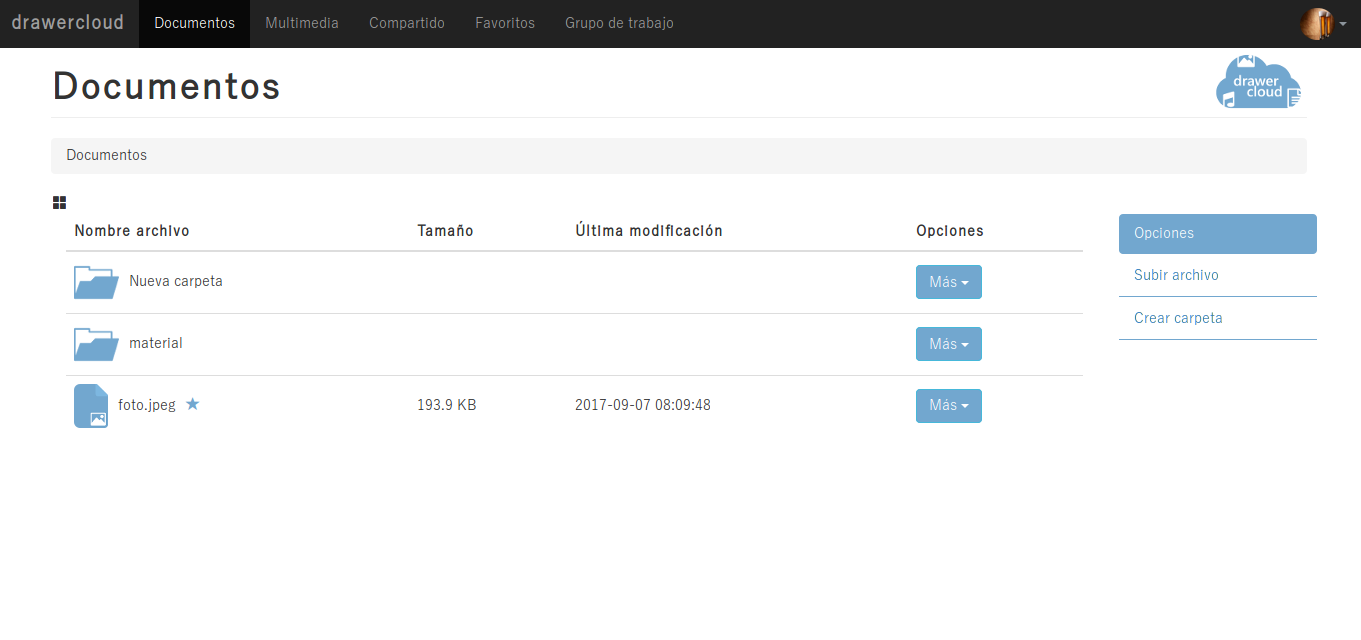
\includegraphics[width=1\textwidth]{imagenes/documentos}
	\caption{Documentos. Aspecto de la página principal}
	\label{fig:documentos}
\end{figure}

\begin{figure}[H]
	\centering
	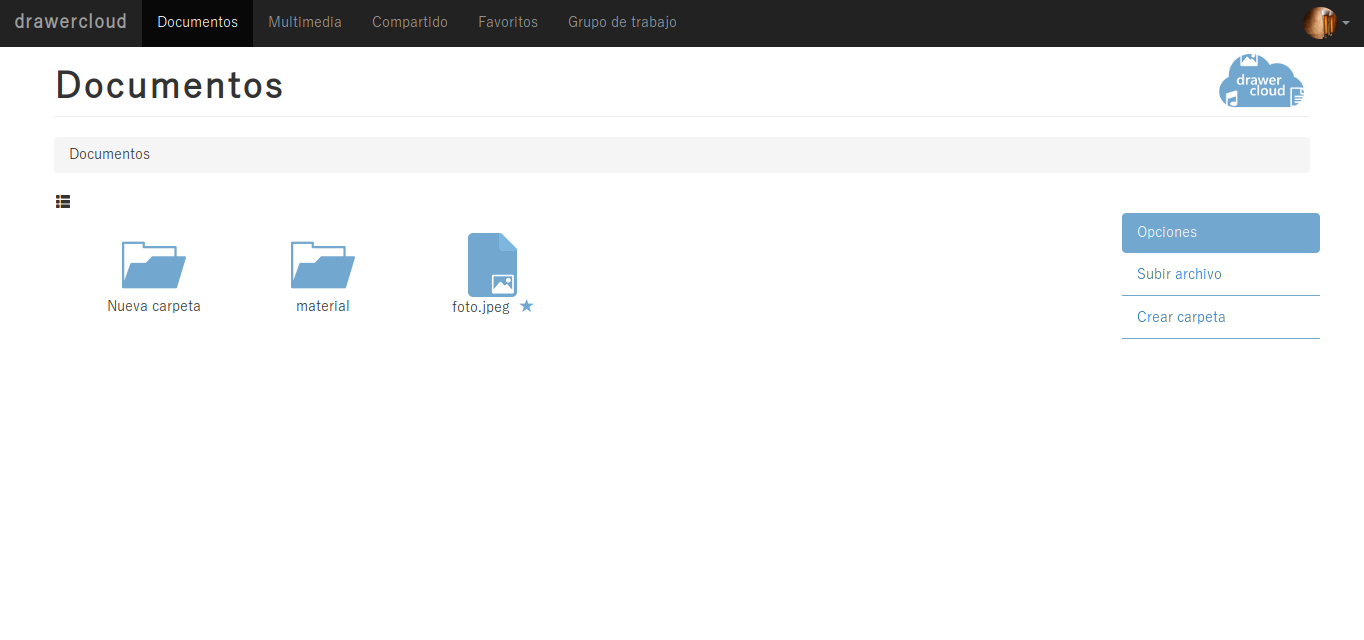
\includegraphics[width=1\textwidth]{imagenes/documentos_iconos}
	\caption{Documentos. Aspecto de la página principal}
	\label{fig:documentos_iconos}
\end{figure}

En \textbf{Documentos} vamos a poder almacenar los archivos que deseemos, podiendo organizar tales archivos en directorios. Para \textbf{crear directorios} o \textbf{subir archivos} hacemos uso de las opciones que aparecen a la derecha de la página documentos \ref{fig:opciones_documentos}.

\begin{figure}[H]
	\centering
	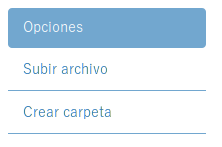
\includegraphics[width=0.4\textwidth]{imagenes/opciones_documentos}
	\caption{Documentos. Opciones de la página Documentos}
	\label{fig:opciones_documentos}
\end{figure}

Los archivos y directorios disponen de \textbf{funcionalidades} propias, como la posibilidad de descargar un archivo, copiar un directorio, etc. Para acceder a estas opciones podemos elegir entre hacer \textbf{click derecho} sobre los directorios/archivos o seleccionar el botón \textbf{Más} disponible para la vista lista.

\subsection{Opciones para archivos}
\begin{itemize}
	\item \textbf{Descargar:} permite transferir el archivo desde la nube hasta el dispositivo usado.
	\item \textbf{Compartir:} dar permisos de lectura sobre el archivo a otro usuario.
	\item \textbf{Cambiar nombre:} renombrar un archivo.
	\item \textbf{Copiar en:} realiza una copia de un archivo.
	\item \textbf{Mover a:} mueve el archivo a otro directorio.
	\item \textbf{Añadir a favoritos:} destaca el archivo sobre el resto.
	\item \textbf{Eliminar:} borra de la nube todos los datos relacionados con el archivo.
\end{itemize} 

\subsection{Opciones para directorios}
\begin{itemize}
	\item \textbf{Cambiar nombre:} renombrar un directorio.
	\item \textbf{Copiar en:} realiza una copia de un directorio.
	\item \textbf{Mover a:} mueve el directorio a otro directorio.
	\item \textbf{Eliminar:} borra de la nube el directorio y todo su contenido.
\end{itemize}

\section{Multimedia}
El apartado \textbf{Multimedia} consta de 3 grupos distintos de archivos multimedia: \textbf{Música, Imágenes y Vídeos} \ref{fig:multimedia}. El contenido de estas carpetas se actualiza de forma automática con la subida de un nuevo fichero. Seleccionando cualquiera de los grupos accederemos a su tipo de contenido.

\begin{figure}[H]
	\centering
	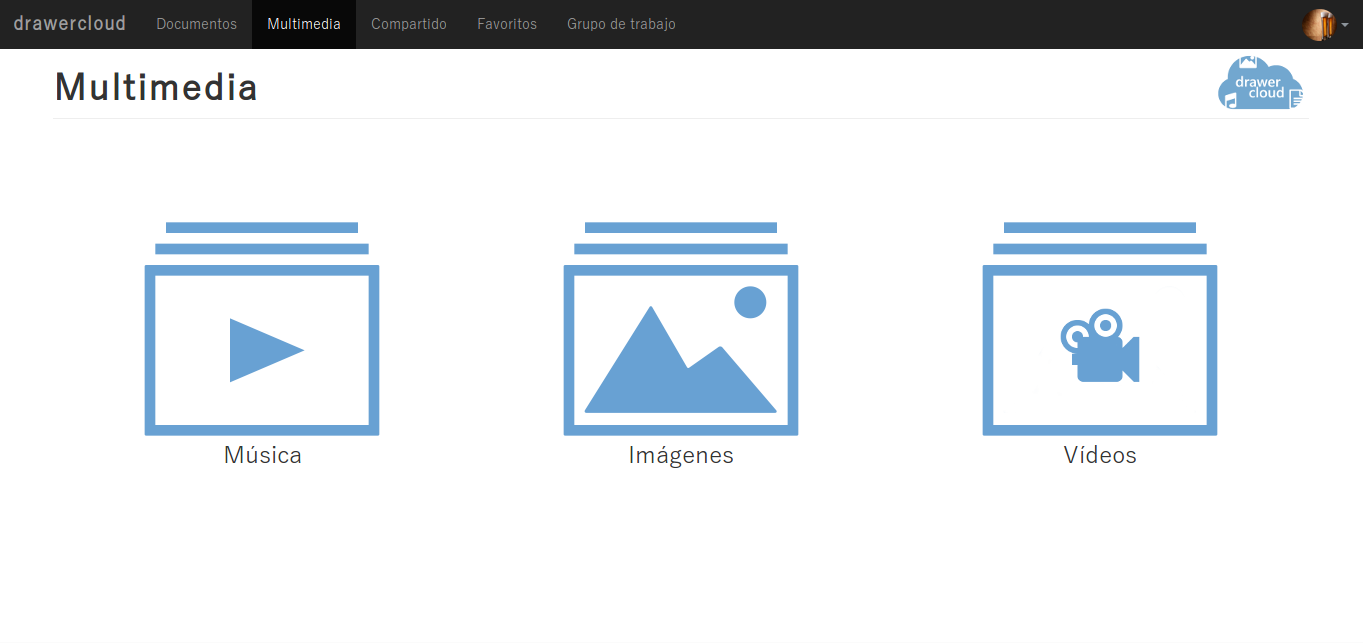
\includegraphics[width=1\textwidth]{imagenes/multimedia}
	\caption{Multimedia. Selección del tipo de contenido.}
	\label{fig:multimedia}
\end{figure}

Dentro de cada grupo obtendremos una lista de los archivos correspondientes. Por ejemplo, si seleccionamos la carpeta imágenes nos encontraremos con todos los archivos de dicho tipo. En esta carpeta volveremos a encontrarnos con las opciones de crear carpeta y subir archivos \ref{fig:opciones_documentos} y las mismas acciones sobre archivos y directorios (copiar, descargar, etc).

\section{Compartir}
\textbf{Compartir} es la página que se encarga de mostrar los archivos que están siendo compartidos. Para mostrar tales archivos se ha dividido la página en dos partes: \textbf{Archivos compartidos por mi} \ref{fig:compartido_por_mi} y \textbf{Archivos compartidos conmigo} \ref{fig:compartido_conmigo}.

\begin{figure}[H]
	\centering
	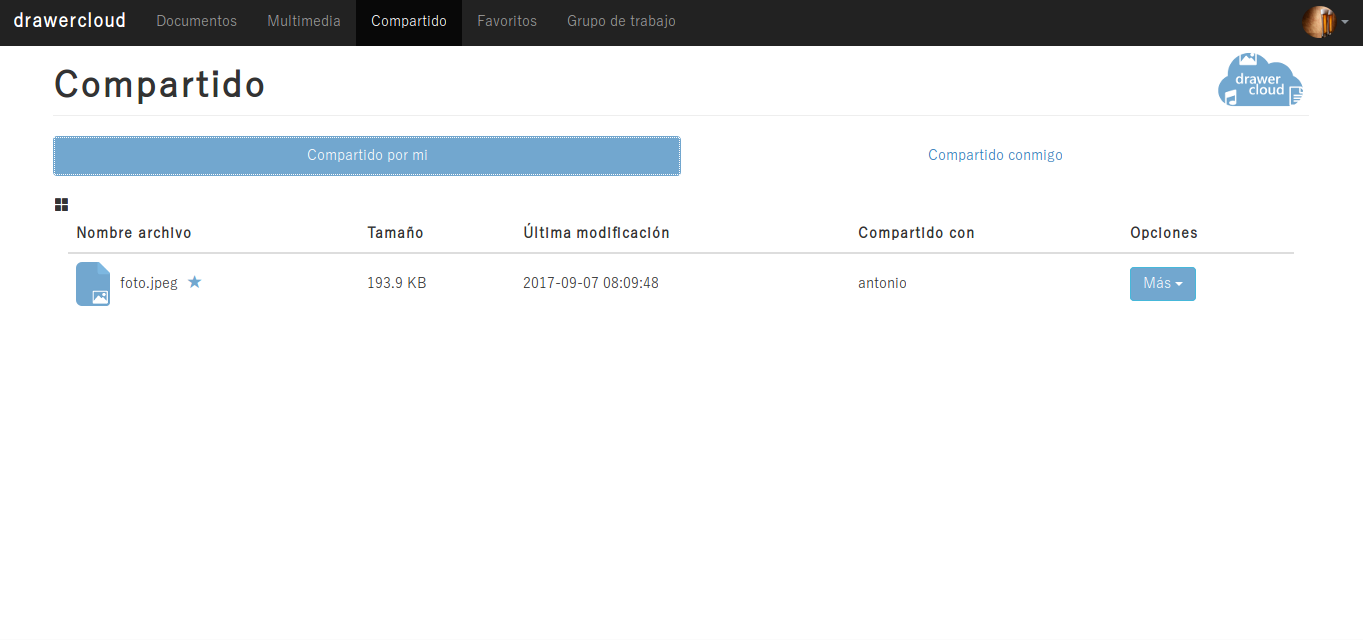
\includegraphics[width=1\textwidth]{imagenes/compartido_por_mi}
	\caption{Compartir. Archivos compartidos por mi.}
	\label{fig:compartido_por_mi}
\end{figure}

\begin{figure}[H]
	\centering
	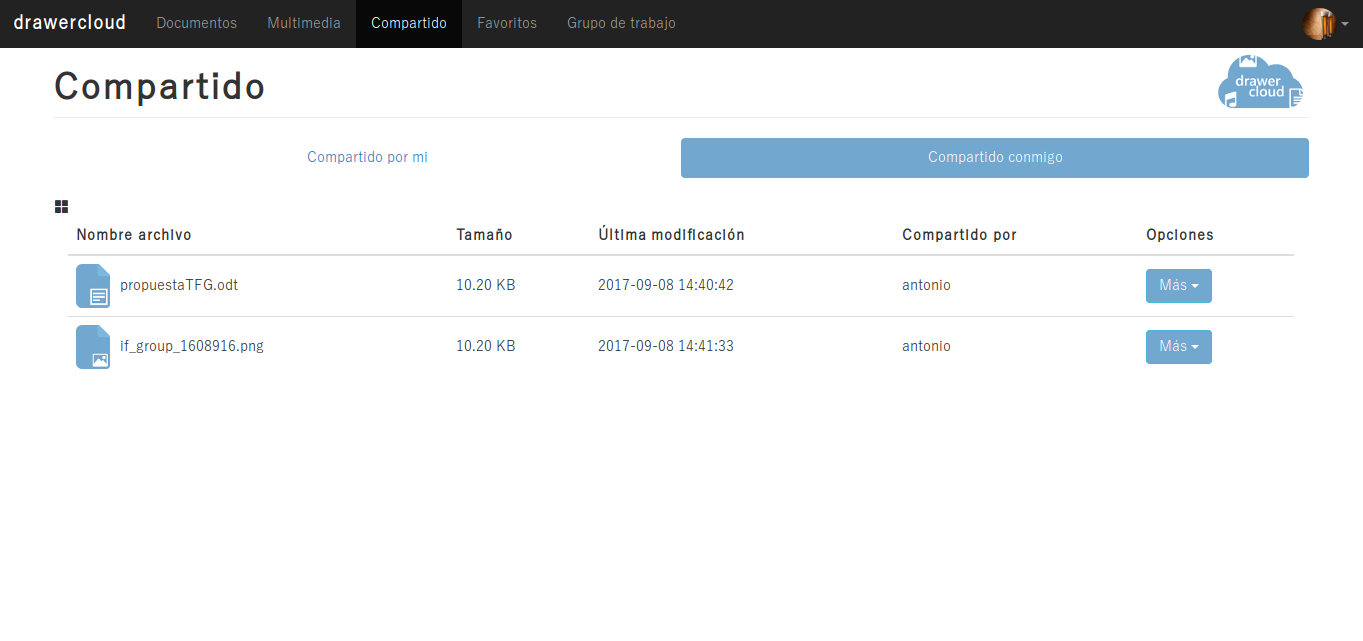
\includegraphics[width=1\textwidth]{imagenes/compartido_conmigo}
	\caption{Compartir. Archivos compartidos conmigo.}
	\label{fig:compartido_conmigo}
\end{figure}

Los archivos realizarán acciones distintas según el apartado en el que estemos. Vemos a continuación que se puede realizar según si es compartido por mi o compartido conmigo.

\subsection{Opciones para archivos compartidos por mi}
\begin{itemize}
	\item \textbf{Descargar:} permite transferir el archivo desde la nube hasta el dispositivo usado.
	\item \textbf{Dejar de compartir:} retira los permisos de lectura sobre el archivo a otro usuario.
	\item \textbf{Cambiar nombre:} renombrar un archivo.
	\item \textbf{Añadir a favoritos:} destaca el archivo sobre el resto.
\end{itemize} 

\subsection{Opciones para archivos compartidos conmigo}
\begin{itemize}
	\item \textbf{Descargar:} permite transferir el archivo desde la nube hasta el dispositivo usado.
	\item \textbf{Dejar de compartir:} nos retira los permisos de lectura sobre el archivo.
	\item \textbf{Añadir a mi nube:} nos permite realizar una copia del archivo en nuestra propia cuenta y nos convierte en propietario de ella.
\end{itemize}

\section{Favoritos}
En la página \textbf{Favoritos} \ref{fig:favoritos} tenemos los archivos que, como el propio nombre de la página indica, han sido marcados como favoritos. Esto nos permite acceder de forma rápida al contenido que hayamos dotado de esta propiedad.

\begin{figure}[H]
	\centering
	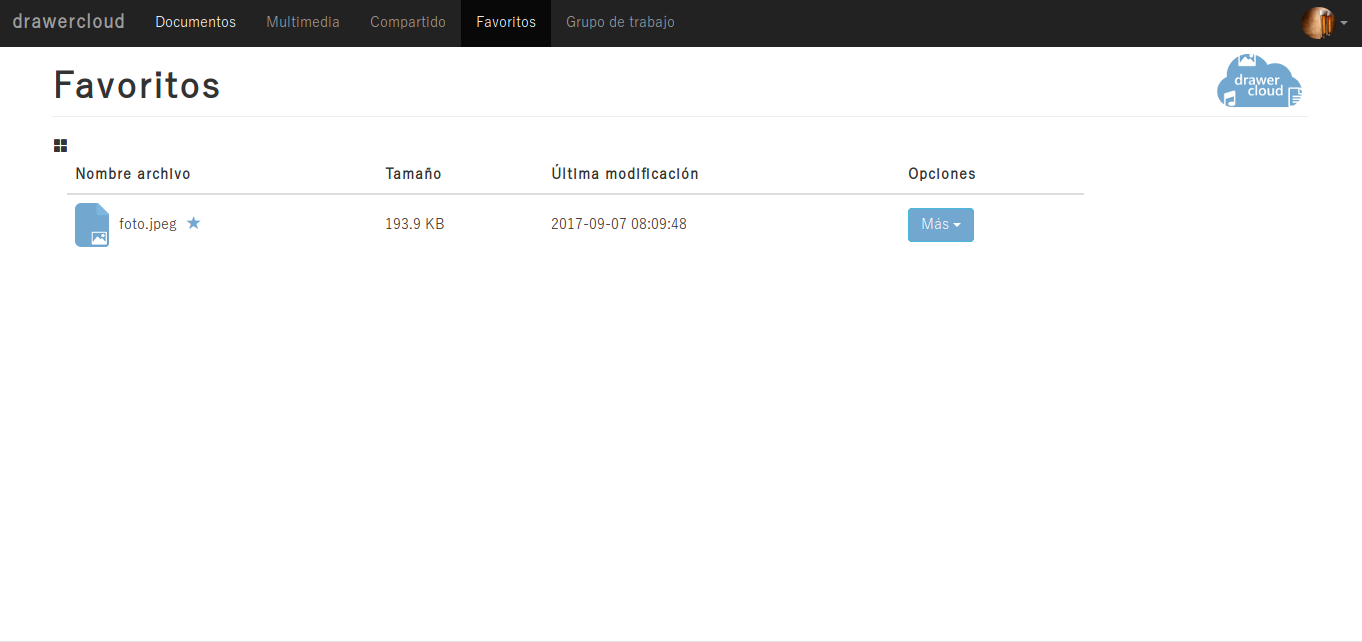
\includegraphics[width=1\textwidth]{imagenes/favoritos}
	\caption{Favoritos. Archivos marcados como favoritos.}
	\label{fig:favoritos}
\end{figure}

Las acciones que los archivos podrán realizar desde este apartado son las siguientes: 

\subsection{Opciones para archivos favoritos}
\begin{itemize}
	\item \textbf{Descargar:} permite transferir el archivo desde la nube hasta el dispositivo usado.
	\item \textbf{Compartir:} dar permisos de lectura sobre el archivo a otro usuario.
	\item \textbf{Cambiar nombre:} renombrar un archivo.
	\item \textbf{Eliminar de favoritos:} elimina la condición de favorito del archivo.
\end{itemize}

\section{Grupo de trabajo}
Por último tenemos la página \textbf{Grupo de trabajo}. Esta sección ha sido creada con el objetivo de crear espacios comunes para distintos usuarios, de modo que todos los participantes del grupo tienen los mismos permisos sobre éste. La primera página que nos aparece al acceder a los grupos de trabajo \ref{fig:grupo_trabajo_principal} nos da a elegir entre \textbf{Ver mis grupos} o \textbf{Crear un grupo}.

\begin{figure}[H]
	\centering
	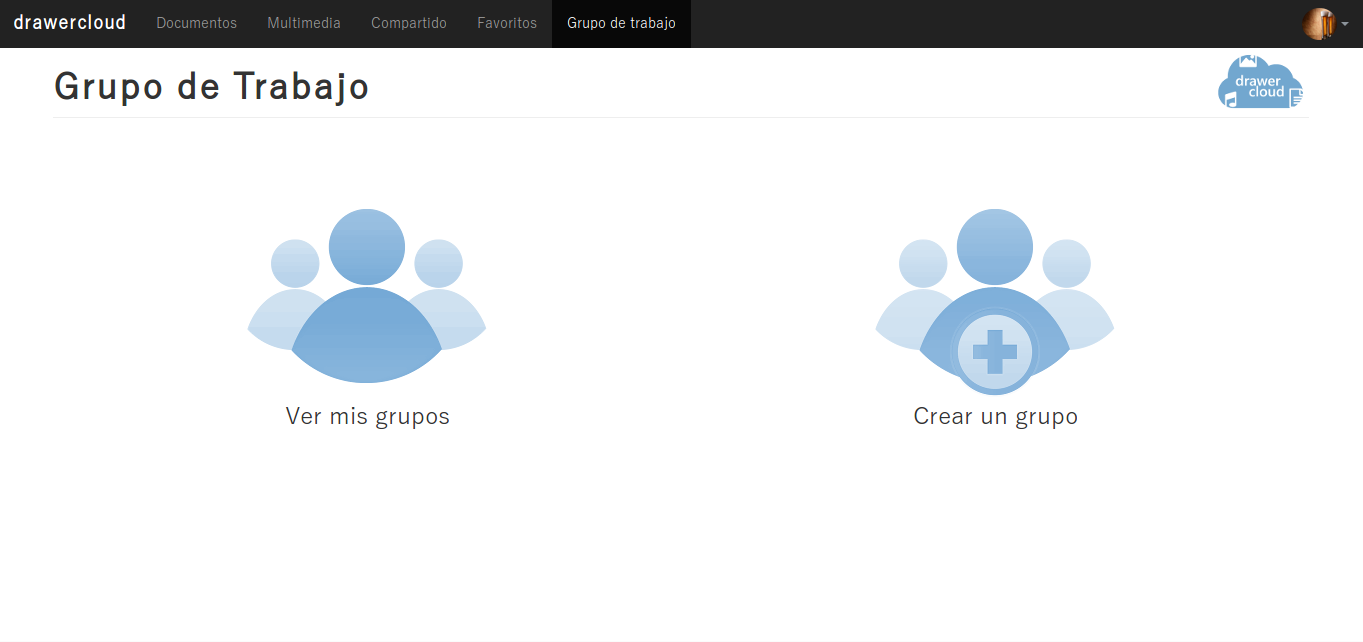
\includegraphics[width=1\textwidth]{imagenes/grupo_trabajo_principal}
	\caption{Grupo de trabajo. Ver mis grupos o Crear un grupo.}
	\label{fig:grupo_trabajo_principal}
\end{figure}

\subsection{Crear un grupo}
Si hemos elegido la opción \textbf{Crear un grupo}, nos aparecerá una ventana como la que vemos en la imagen \ref{fig:crear_grupo}. En la ventana emergente indicaremos el nombre del grupo y pulsaremos en \textbf{Crear grupo} para finalizar.

\begin{figure}[H]
	\centering
	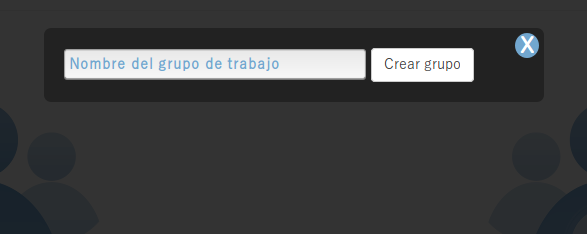
\includegraphics[width=1\textwidth]{imagenes/crear_grupo}
	\caption{Grupo de trabajo. Crear un grupo.}
	\label{fig:crear_grupo}
\end{figure}

\subsection{Ver mis grupos}
Si por el contrario hemos elegido la opción \textbf{Ver mis grupos}, nos aparecerá una ventana como la que vemos en la imagen \ref{fig:ver_mis_grupos}. En la ventana emergente nos aparece una lista con los grupos a los que pertenecemos. Accederemos al interior de cada grupo haciendo click sobre el elegido.

\begin{figure}[H]
	\centering
	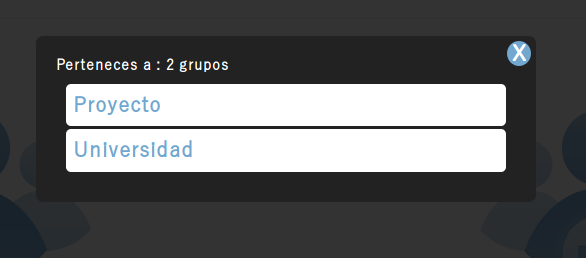
\includegraphics[width=1\textwidth]{imagenes/ver_mis_grupos}
	\caption{Grupo de trabajo. Ver mis grupos.}
	\label{fig:ver_mis_grupos}
\end{figure}


\subsection{Contenido de un grupo de trabajo}
Una vez hemos accedido a un grupo de trabajo veremos algo similar a lo que nos muestra la figura \ref{fig:grupo_trabajo}. Contamos de nuevo con la estructura repetida en las otras páginas: una arquitectura de archivos y directorios (mostrados en lista o iconos) y las posibles acciones en un menú a la derecha.

\begin{figure}[H]
	\centering
	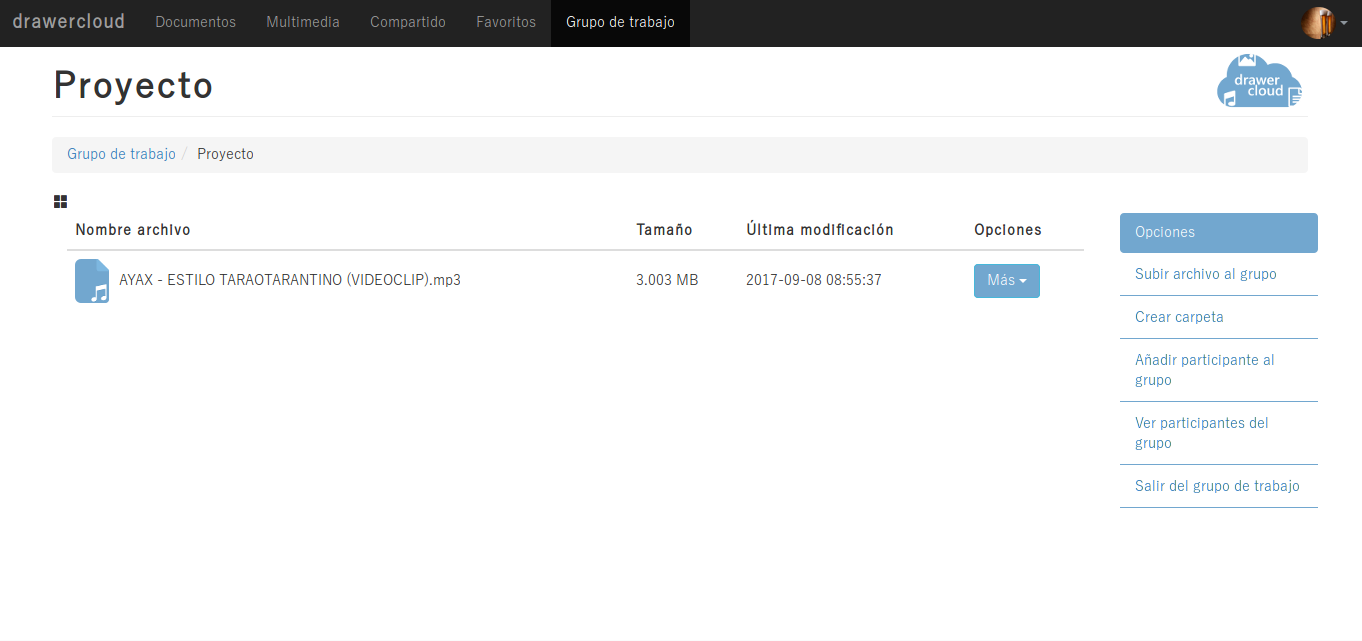
\includegraphics[width=1\textwidth]{imagenes/grupo_trabajo}
	\caption{Grupo de trabajo. Contenido de un grupo de trabajo.}
	\label{fig:grupo_trabajo}
\end{figure}

Comentamos a continuación las acciones posibles a realizar en un grupo de trabajo \ref{fig:opciones_grupo_trabajo}:

\begin{figure}[H]
	\centering
	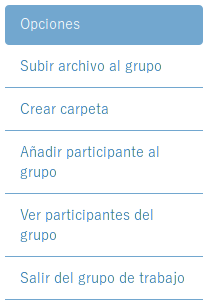
\includegraphics[width=0.3\textwidth]{imagenes/opciones_grupo_trabajo}
	\caption{Grupo de trabajo. Opciones de un grupo de trabajo.}
	\label{fig:opciones_grupo_trabajo}
\end{figure}

\begin{itemize}
	\item \textbf{Subir archivo al grupo:} seleccionamos un archivo en el dispositivo usado y lo añadimos a nuestro grupo. Todos los participantes tendrán los mismos permisos sobre él.
	\item \textbf{Crear carpeta:} añade un directorio al grupo de trabajo.
	\item \textbf{Añadir participante al grupo:} añade un participante al grupo de trabajo.
	\item \textbf{Ver participantes del grupo:} muestra una lista con los participantes del grupo de trabajo.
	\item \textbf{Salir del grupo de trabajo:} el usuario deja de ser un participante del grupo. Cuando el grupo queda sin participantes, se elimina automáticamente junto con todo su contenido.
\end{itemize}

\subsubsection{Opciones para los archivos dentro de un grupo de trabajo:}
\begin{itemize}
	\item \textbf{Descargar:} permite transferir el archivo desde la nube hasta el dispositivo usado.
	\item \textbf{Cambiar nombre:} renombrar un archivo.
	\item \textbf{Copiar en:} realiza una copia de un archivo.
	\item \textbf{Mover a:} mueve el archivo a otro directorio.
	\item \textbf{Eliminar:} borra de la nube todos los datos relacionados con el archivo.
\end{itemize}

\subsubsection{Opciones para los directorios dentro de un grupo de trabajo:}
\begin{itemize}
	\item \textbf{Cambiar nombre:} renombrar un directorio.
	\item \textbf{Copiar en:} realiza una copia de un directorio.
	\item \textbf{Mover a:} mueve el directorio a otro directorio.
	\item \textbf{Eliminar:} borra de la nube el directorio y todo su contenido.
\end{itemize} 

\section{Opciones de usuario}
Si nos fijamos, en la esquina superior derecha nos aparece un icono con nuestra imagen de perfil y una flechita a su derecha. Pulsando sobre tal icono nos muestra otra lista de opciones que vemos en la figura \ref{fig:opciones_usuarios}.

\begin{figure}[H]
	\centering
	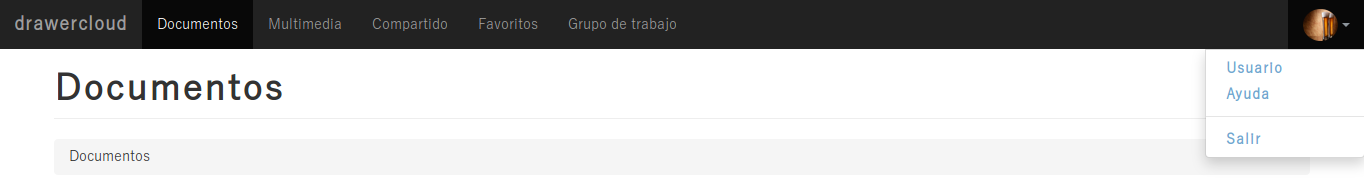
\includegraphics[width=1\textwidth]{imagenes/opciones_usuarios}
	\caption{Opciones de usuario.}
	\label{fig:opciones_usuarios}
\end{figure}

\subsection{Usuario}
El apartado \textbf{Usuario} muestra información referente al cliente \ref{fig:usuario}. Desde esta sección podremos consultar información sobre nuestra cuenta, cambiar nuestra imagen de perfil (haciendo click sobre la propia imagen) o eliminar la cuenta.

\begin{figure}[H]
	\centering
	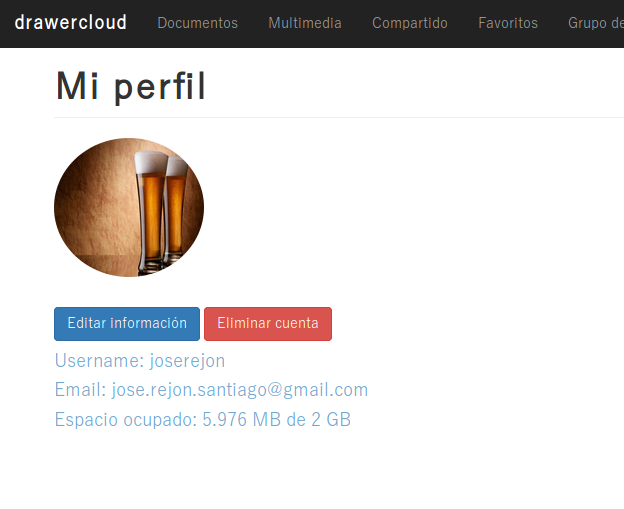
\includegraphics[width=1\textwidth]{imagenes/usuario}
	\caption{Opciones de usuario. Usuario.}
	\label{fig:usuario}
\end{figure}

\subsection{Ayuda}
La página de \textbf{Ayuda} \ref{fig:ayuda} detalla las acciones posibles que puede realizar el usuario en cada apartado. Para elegir entre los distintos apartados desplegamos el botón \textbf{Ayuda} y seleccionamos el tema sobre el que queremos recibir información.

\begin{figure}[H]
	\centering
	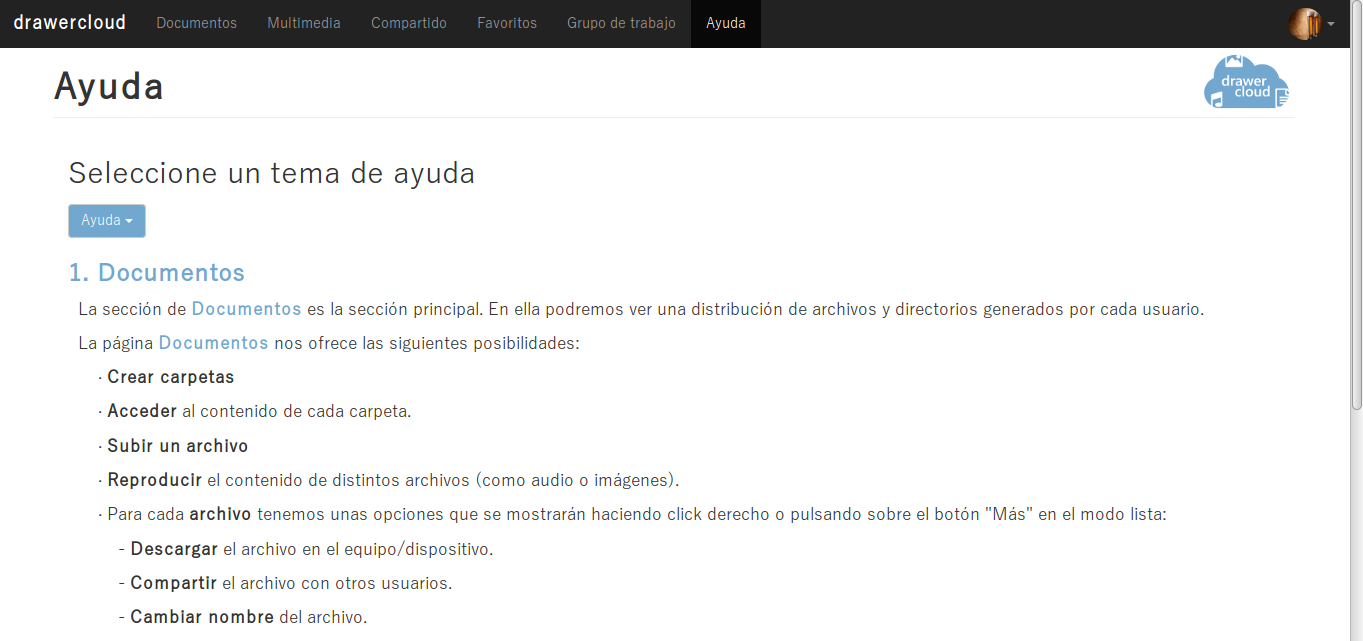
\includegraphics[width=1\textwidth]{imagenes/ayuda}
	\caption{Opciones de usuario. Ayuda.}
	\label{fig:ayuda}
\end{figure}

\subsection{Salir}
Pulsando en \textbf{Salir} cerramos la sesión actual y volvemos a la página de login.